% \documentclass[handout]{beamer}
\documentclass[presentation]{beamer}
\usepackage[utf8]{inputenc}
\usepackage{amsmath}
\usepackage{xcolor}
\usepackage{listings}
\usepackage{hyperref}
\usepackage{graphicx}
\usepackage{tikz}
\usepackage[T1]{fontenc}
\usepackage[utf8]{inputenc}
% \usepackage{colortbl}
% \usepackage{caption}
% \usepackage{textcomp}
% \usepackage{arioref}
% \usepackage{afterpage}
% \usepackage{subcaption}
% \usepackage{float}
% \usepackage{bm}
% \usepackage{amssymb}
% \usepackage{pdfpages}
% \usepackage{pdflscape}
% \usepackage{lscape}

% Change font
% \usepackage{fontspec}
% \defaultfontfeatures{Mapping=tex-text,Scale=MatchLowercase}
% \setmainfont{Ubuntu}
% \setmonofont{Ubuntu Mono}


%%%%%%%%%%%%%%%%%%%%%%%%%%%
%   Beamer customization  %
%%%%%%%%%%%%%%%%%%%%%%%%%%%

\newcommand{\gooditem}[1]{\setbeamercolor{item}{fg=green}\item #1}
\newcommand{\baditem}[1]{\setbeamercolor{item}{fg=red}\item #1}


\setbeamertemplate{blocks}[rounded][shadow=false]


\usefonttheme[onlysmall]{structurebold}
% Use a bold face title font
\setbeamerfont{title}{series=\bfseries}
\setbeamerfont{frametitle}{series=\bfseries}

\setbeamercolor{frametitle}{fg=black!65!white,bg=white}
\setbeamercolor{normal text}{fg=black!75!white,bg=white}
\setbeamercolor{structure}{fg=black,bg=white}


% Suppress navigation symbols
\setbeamertemplate{navigation symbols}{}

\definecolor{myred}{RGB}{190,0,0}


\graphicspath{{./figures/}}


%%%%%%%%%%%%%%
%   Colors   %
%%%%%%%%%%%%%%


\definecolor{logogrey}{HTML}{426E86}
\definecolor{logored}{HTML}{E50000}
\definecolor{logoyellow}{HTML}{F9BA32}


%%%%%%%%%%%%%%%%
%   Commands   %
%%%%%%%%%%%%%%%%

\newcommand{\fullimage}[2]{
  \begin{tikzpicture}[remember picture, overlay]
    \node[anchor = center] (image) at (current page.center) {\includegraphics[scale=#2]{#1}};
  \end{tikzpicture}
}


%%%%%%%%%%%%%%%%%%%%%%%%%%%%%%%%
%   lstlistings customization  %
%%%%%%%%%%%%%%%%%%%%%%%%%%%%%%%%



\definecolor{listingsstringcolor}{rgb}{0.7294117647058823, 0.12941176470588237, 0.12941176470588237}
\definecolor{listingskeywordcolor}{rgb}{0.0,0.5,0.0}
\definecolor{listingsbasiccolor}{rgb}{0.0,0.0,0.0}
\definecolor{listingsnumbercolor}{rgb}{0.53, 0.53, 0.53}
\definecolor{listingscommentcolor}{rgb}{0.25,0.5,0.5}
\definecolor{listingsbackgroundcolor}{rgb}{0.9686274509803922, 0.9686274509803922, 0.9686274509803922}
\definecolor{listingsrulecolor}{rgb}{0.8117647058823529, 0.8117647058823529, 0.8117647058823529}
\definecolor{listingsidentifiercolor}{rgb}{0.0,0.0,0.0}
\definecolor{listingsclasscolor}{rgb}{0.0,0.5,0.0}
\definecolor{listingsmembercolor}{rgb}{0.5,0.0,0.0}
\definecolor{listingsdirectivecolor}{rgb}{0.0,0.0,0.5}
\definecolor{pyoutbackground}{rgb}{1.0, 1.0, 1.0}
\definecolor{pyoutrule}{rgb}{.25882353,  0.64705882,  0.96078431}
\definecolor{pseudobackground}{RGB}{227,  248,  255}


\lstset {
    language=Python,
    otherkeywords={self},
    keywordstyle=\ttfamily\color{blue!90!black},
    keywords=[2]{True,False},
    keywords=[3]{ttk},
    keywordstyle={[2]\ttfamily\color{yellow!80!orange}},
    keywordstyle={[3]\ttfamily\color{red!80!orange}},
    emph={MyClass,__init__},
    emphstyle=\ttfamily\color{red!80!black},
    stringstyle=\color{green!80!black},
    showstringspaces=false
    backgroundcolor=\color{listingsbackgroundcolor},
    frame=lrtb,                    % adds a frame around the code
    framexleftmargin=5pt,
    framexrightmargin=5pt,
    framextopmargin=0pt,
    framexbottommargin=0pt,
    xleftmargin=9pt,
    xrightmargin=9pt,
    rulecolor=\color{listingsrulecolor},
    tabsize=4,                       % sets default tabsize to 2 spaces
    showstringspaces=false,
    captionpos=b,
    escapeinside={(*@}{@*)},
    keywords=[2]{True,False},
    basicstyle=\color{listingsbasiccolor}\ttfamily,
    keywordstyle=\color{listingskeywordcolor}\ttfamily\bfseries,
%    directivestyle=\color{listingsdirectivecolor}\ttfamily,
    stringstyle=\color{listingsstringcolor}\ttfamily,
    commentstyle=\color{listingscommentcolor}\ttfamily,
    numberstyle=\color{listingsnumbercolor}\ttfamily,
    identifierstyle=\color{listingsidentifiercolor}\ttfamily,
    keywordstyle=[2]{\color{listingsclasscolor}\ttfamily},
    keywordstyle=[3]{\color{listingsmembercolor}\ttfamily},
    keywordstyle=[4]{\color{listingsdirectivecolor}\ttfamily},
}






\begin{document}



%%%%%%%%%%%%%
%   Frame   %
%%%%%%%%%%%%%

\begin{frame}
% \begin{center}
    \textbf{\color{myred}\Large How to model effects of uncertain model parameters with Uncertainpy}
% \end{center}

     \large \vspace{8mm} Simen Tennøe

      \vspace{6mm}
      \scriptsize Supervisors:

    %
      \vspace{1mm}

      Gaute Einevoll

      Geir Halnes

      \vspace{15mm}
    \small University of Oslo, CINPLA
 %
 \begin{tikzpicture}[remember picture,overlay]
    \node [xshift=0.19\paperwidth,yshift=-0.14\paperheight] at (current page.center)
          {\includegraphics[width = 0.375\paperwidth ]{uncertainpy_small.pdf}};
  \end{tikzpicture}

  \begin{tikzpicture}[remember picture,overlay]
    \node [xshift=1.35cm,yshift=0.55cm] at (current page.south west)
          {\includegraphics[width = 0.2\paperwidth ]{cinpla.png}};
  \end{tikzpicture}

\end{frame}



%%%%%%%%%%%%%
%   Frame   %
%%%%%%%%%%%%%


% \begin{frame}[fragile]{UncertainPy is a Python toolbox for uncertainty quantification of computation neuroscience models}


%     \begin{tikzpicture}[remember picture, overlay, font=\sffamily]
%       \node [align=left, xshift=-0.4\textwidth,yshift=0.15\textwidth] (image3) at (current page.center)
%             {\includegraphics[width = 0.2\textwidth]{chaospy_logo.jpg}};
%       \node[align=left] at (image3.east) {\hspace{5cm} \bf Properties of Chaospy};
%     \end{tikzpicture}

%   \pause

%   \begin{tikzpicture}[remember picture, overlay, font=\sffamily]
%   \node [align=left, xshift=-0.2\textwidth,yshift=-0.05\textwidth] (image1) at (current page.center)
%       {\includegraphics[width = 0.25\textwidth]{samples.png}};
%   \node[align=left] at (image1.east) {\hspace{4.5cm} \bf Monte Carlo methods};
%   \end{tikzpicture}

% \pause


%     \begin{tikzpicture}[remember picture, overlay, font=\sffamily]
%       \node [align=left, xshift=0\textwidth,yshift=-0.25\textwidth] (image2) at (current page.center)
%             {\includegraphics[width = 0.25\textwidth]{pc.png}};
%       \node[align=left] at (image2.east) {\hspace{4cm} \bf Polynomial Chaos};
%     \end{tikzpicture}

% \end{frame}

%%%%%%%%%%%%%
%   Frame   %
%%%%%%%%%%%%%

\begin{frame}{Computational models contain parameters}
  % \[I = C_m\frac{{\mathrm d} V_m}{{\mathrm d} t}  + {\bf\color{logogrey}I_{K}} + {\bf\color{logoyellow}I_{Na}} + {\bf\color{logored}I_{l}}\]

  % \vspace{-5mm}
  \begin{figure}
    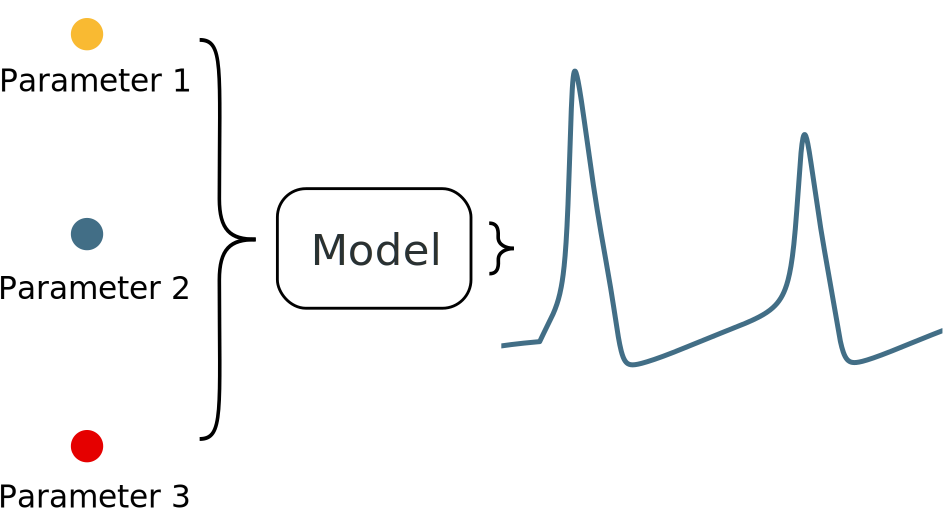
\includegraphics[width=\textwidth]{deterministic.png}
  \end{figure}

\end{frame}




\begin{frame}{Example: the Hodgkin-Huxley model}
  % \[I = C_m\frac{{\mathrm d} V_m}{{\mathrm d} t}  + I_{K} + I_{Na} +I_{l}\]
 \LARGE  \[I = C_m\frac{{\mathrm d} V_m}{{\mathrm d} t}  + {\bf\color{logogrey}I_{K}} + {\bf\color{logoyellow}I_{Na}} + {\bf\color{logored}I_{l}}\]

\end{frame}


%%%%%%%%%%%%%
%   Frame   %
%%%%%%%%%%%%%

\begin{frame}

  \begin{figure}
    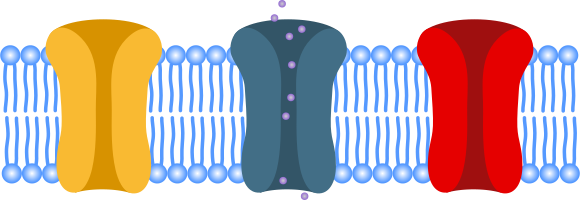
\includegraphics[width=\textwidth]{deterministic_channels.png}
  \end{figure}
\end{frame}


%%%%%%%%%%%%%
%   Frame   %
%%%%%%%%%%%%%

\begin{frame}{Example: the Hodgkin-Huxley model}
  \begin{figure}
    \includegraphics[width=\textwidth]{hh_single.png}
  \end{figure}

\end{frame}




%%%%%%%%%%%%%
%   Frame   %
%%%%%%%%%%%%%

\begin{frame}{Changing parameters give different results}
\[I = C_m\frac{{\mathrm d} V_m}{{\mathrm d} t}  + {\bf\color{logogrey}I_{K}} + {\bf\color{logoyellow}I_{Na}} + {\bf\color{logored}I_{l}}\]


  \begin{figure}
    \includegraphics[height=0.7\textheight]{hh.png}
  \end{figure}

\end{frame}

% %%%%%%%%%%%%%
% %   Frame   %
% %%%%%%%%%%%%%

% \begin{frame}{Problem: The parameters are uncertain}
%   \begin{figure}
%     \only<1>{\includegraphics[width=1\textwidth]{not_deterministic.png}}
%     \only<2>{\includegraphics[width=1\textwidth]{not_deterministic_distributions.png}}
%   \end{figure}

% \end{frame}


%%%%%%%%%%%%%
%   Frame   %
%%%%%%%%%%%%%

\begin{frame}{Problem: The parameters are uncertain}
  \begin{figure}
    \includegraphics[width=1\textwidth]{not_deterministic_channels.png}
  \end{figure}

\end{frame}



%%%%%%%%%%%%%
%   Frame   %
%%%%%%%%%%%%%

% \begin{frame}[plain]{\color{black}Measurement uncertainty}

% \begin{tikzpicture}[remember picture, overlay]
%   \node[anchor = center] (image) at (current page.center) {\includegraphics[scale=0.38]{eeg.jpg}};
%   \node[align = left, xshift=0.4cm, yshift=-0.4cm] at (current page.135) {\bf Measurement uncertainty};
% \end{tikzpicture}

% \end{frame}

\begin{frame}{Cause of uncertainty: measurement uncertainty}

  \begin{figure}

    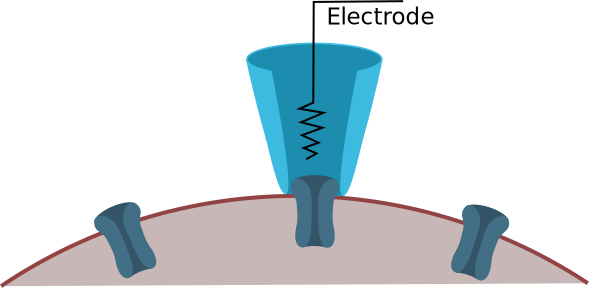
\includegraphics[height=0.9\textheight]{patch_clamp.png}
  \end{figure}

\end{frame}



%%%%%%%%%%%%%
%   Frame   %
%%%%%%%%%%%%%

\begin{frame}{Cause of uncertainty: biological variability}
  \begin{figure}
    \only<1>{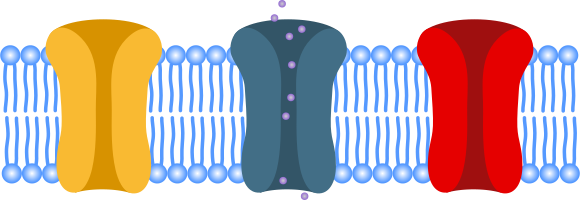
\includegraphics[width=1\textwidth]{channels.jpg}}
    \only<2>{\includegraphics[width=1\textwidth]{neurons.jpg}}
  \end{figure}

\end{frame}





%%%%%%%%%%%%%
%   Frame   %
%%%%%%%%%%%%%

\begin{frame}{Parameters are best described by distributions}
  \begin{figure}
    \includegraphics[width=1\textwidth]{distribution_channels.png}
  \end{figure}

\end{frame}




%%%%%%%%%%%%%
%   Frame   %
%%%%%%%%%%%%%

\begin{frame}{Uncertainty quantification is the process of quantifying the effects of
              uncertain input parameters}
  \begin{figure}
    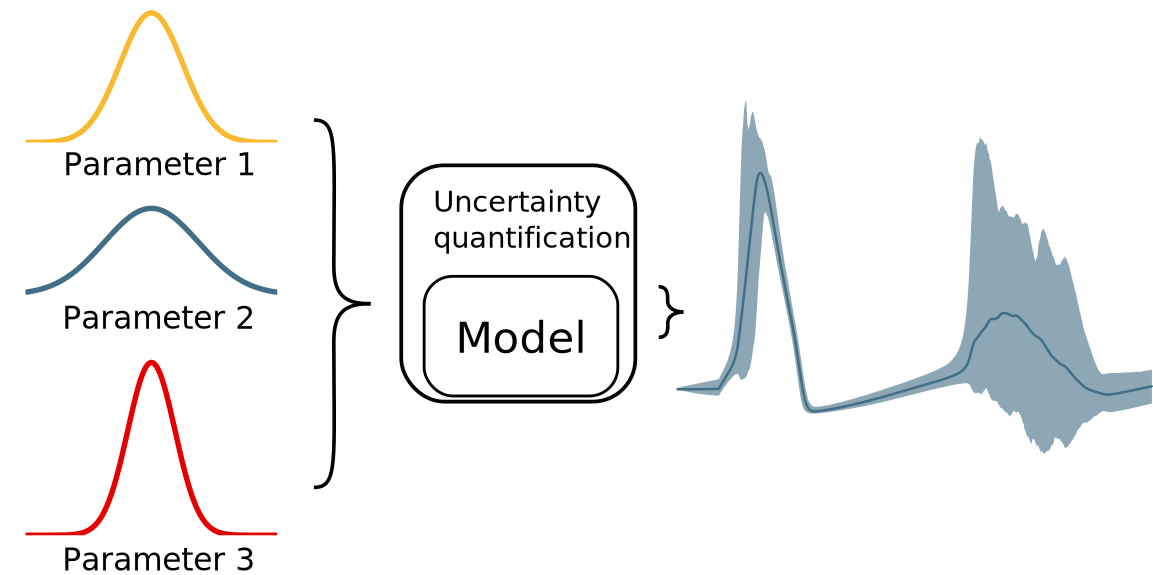
\includegraphics[width=1\textwidth]{probabalistic.png}
  \end{figure}

\end{frame}





\end{document}